\documentclass[english,11pt]{article}
\usepackage[table]{xcolor}
\usepackage{color}
\usepackage{amsmath}
\usepackage{amsmath}
\usepackage{amssymb}
\usepackage{color}
\usepackage{tikz,graphicx}
\usetikzlibrary{positioning,arrows.meta,calc,decorations.pathreplacing}

\begin{document}

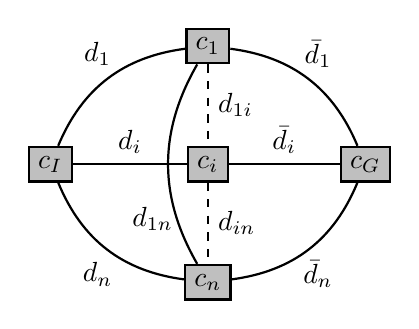
\begin{tikzpicture}[thick,scale=1]
     % Villes
  \node[draw, fill=black!25] (0) at (-2,0) {$c_I$};
  \node[draw, fill=black!25] (1) at (0,1.5) {$c_1$};
  \node[draw, fill=black!25] (2) at (0,0) {$c_i$};
  \node[draw, fill=black!25] (3) at (0,-1.5) {$c_n$};
  \node[draw, fill=black!25] (4) at (2,0) {$c_G$};
 
     % Liaison inter villes
  \draw[thick] (0) to[bend left] (1);
  \draw[thick] (0)--(2) node[midway, above]{$d_i$};
  \draw[thick, bend left] (0) to[bend right] (3);
  
  \draw[thick] (1) to[bend left] (4);
  \draw[thick] (2)--(4) node[midway, above]{$\bar d_i$};
  \draw[thick] (3) to[bend right] (4);
  
  \draw[dashed] (1)--(2) node[midway, right]{$d_{1i}$};
  \draw[dashed] (2)--(3) node[midway, right]{$d_{in}$};
  \draw[thick] (1) to[bend right] (3);
     
     % Distance particulière
  \node[] (A) at (-1.4,1.4) {$d_1$};
  \node[] (A) at (1.4,1.4) {$\bar d_1$};
  \node[] (A) at (-1.4,-1.4) {$d_n$};
  \node[] (A) at (1.4,-1.4) {$\bar d_n$};
  \node[] (A) at (-0.7,-0.7) {$d_{1n}$};
  
\end{tikzpicture}

\end{document}